% !TEX root = ../thesis.tex

\chapter{Temporal Ordering of Images \label{ch:drosophila}}

\graphicspath{{ch-drosophila/figures/}}

{\em This work was published in \citep{dsilva2015temporal}}

\section{Introduction}

\begin{figure}[t]
\centering
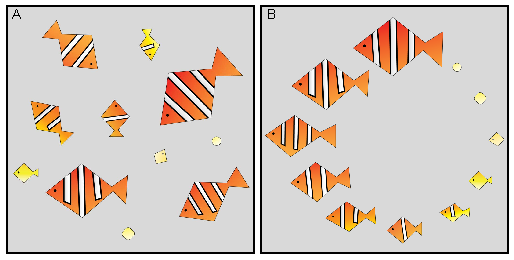
\includegraphics{fig1}
\caption[Caricature illustrating the tasks of image registration and temporal ordering]{Caricature illustrating the tasks of image registration and temporal ordering. (A) Images of ``samples'', each in a different orientation and a different stage of development. (B) Registered and ordered samples. For this caricature, the registration and ordering is straightforward because the data set is small, the landmarks are visually apparent, and the developmental changes are easy to recognize.}
\label{fig:fish}
\end{figure}

In one of the common approaches to studies of developmental dynamics in biology, a group of embryos is fixed and stained to visualize a particular biochemical or morphological process within a developing tissue.
%
The developmental dynamics must then be reconstructed from multiple embryos, each of which contributes only a snapshot of the relevant process along its developmental trajectory \citep{jaeger2004dynamic, peter2011gene, fowlkes2008quantitative}.
%
Importantly, the ``age'' of any given embryo arrested in its development is often only approximately known.
%
Typically, what is known is
a certain time window to which a collection of embryos belongs \citep{ng2012large, richardson2014emage, castro2009automatic}.
%
Furthermore, images are often collected in different spatial orientations.
%
In order to recover the developmental dynamics from such data sets, snapshots of different embryos must first be spatially aligned or {\em registered}, and then ordered in time.


Temporal ordering and registration of images can be done manually
when the number of images is small and the differences between them are visually apparent.
%
\fig~\ref{fig:fish} shows a caricature of fish development which illustrates the processes of growth and patterning.
%
In this case, temporal ordering can be accomplished by arranging the fish by size, which is monotonic with the developmental progress.
%
Image registration is based on obvious morphological landmarks, such as the positions of the head and the fins.
%
In contrast to this example, real data pose nontrivial challenges for both registration and temporal ordering.
%
In general, the landmarks needed for registration, as well as the attributes which can be used to order the data, are not known {\it a priori}.
%
Additional challenges arise from embryo-to-embryo variability, sample size, and measurement noise.

We present a robust algorithmic approach to simultaneous registration and temporal ordering.
%
In contrast to a number of previous methodologies \citep{zitova2003image, rowley1998rotation, hajnal2010medical, greenspan1994rotation, zhao2003face, dubuis2013accurate}, our methodology does not rely on the {\em a priori} knowledge of landmarks for registration or markers of developmental progression.
%
The approach is based on vector diffusion maps \citep{singer2012vector}, a manifold learning algorithm which simultaneously addresses the problems of registration and temporal ordering.
%
This algorithm is one of several nonlinear dimensionality reduction techniques that have been developed over the past decade \citep{Belkin2003, coifman2005geometric, coifman2006geometric, tenenbaum2000global, roweis2000nonlinear}, for
applications ranging from analysis of cryo-electron microscopy (cryo-EM) images of individual molecules  \citep{zhao2014rotationally, singer2011viewing} to face recognition \citep{lafon2006data} and classification of CT scans \citep{fernandez2014diffusion}.

Here, the vector diffusion maps algorithm is adapted for the analysis of images of developing tissues in studies of developmental dynamics, with the main objective of revealing stereotypic developmental trajectories from fixed images.
%
To illustrate our approach, we analyze four experimental data sets.
%
Our first two data sets come from live imaging studies of {\em Drosophila} and zebrafish embryogenesis.
%
In both of these examples, the correct rotational orientation and temporal order are independently known, and these data sets will be used to validate our approach.
%
Our third data set consists of images from fixed {\em Drosophila} embryos where the correct orientation and order is unknown; here, we will show how the algorithm can help uncover developmental dynamics which are not readily apparent.
%
Our final data set consists of z-stacks of {\em Drosophila} wing discs, which we will use to illustrate how our methods can be used to analyze specific types of three-dimensional imaging data.
%
We also show how to compute an average trajectory from a set of registered and ordered fixed images to remove noise due to intersample variability and obtain a smooth description of the underlying developmental dynamics.

\section{Materials and Methods}






\subsection{Vector diffusion maps for registration and temporal ordering}

Vector diffusion maps \citep{singer2012vector} is a manifold learning
technique developed for data sets which contain two sources of variability:
geometric symmetries, such as rotations of the images, which one would like to factor out,
and ``additional" directions of variability, such as temporal dynamics, which one would like to uncover.
%
Vector diffusion maps combine two algorithms, {\em angular synchronization} \citep{singer2011angular} for image registration and {\em diffusion maps} \citep{coifman2005geometric} for extracting intrinsic low-dimensional structure in data, into a single computation.
%
A schematic illustration of the algorithms is shown in \fig~\ref{fig:schematics}, and the details of the algorithms are given in \chap~\ref{ch:math}.
%
We will use the algorithm to register images of developing tissues with respect to planar rotations, as well as uncover the main direction of variability {\it after} removing rotational symmetries.
%
Although in general, images may contain variations due to rotations, translations, and scaling, we will remove the relevant translations and/or scaling via relatively simple image preprocessing, and focus only on factoring out rotations using the vector diffusion maps algorithm.
%
In the case that {\em all} relevant symmetries can be removed with straightforward preprocessing, our algorithms can extract the main direction of variability within the imaging data set.
%
We assume that this main direction of remaining variability in these images is parameterized by the developmental time of each embryo.
%
As a consequence, uncovering this direction should reveal the underlying dynamics.


\begin{figure}[t]
\centering
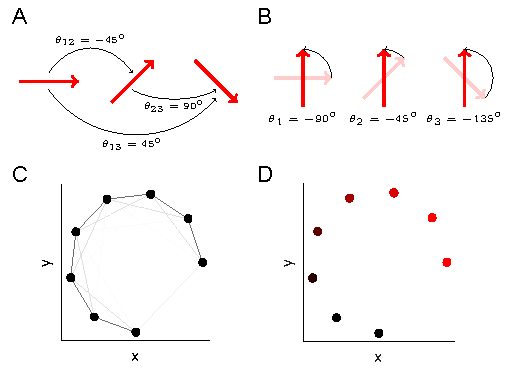
\includegraphics[width=0.7\textwidth]{fig2}
\caption[Schematic illustrating angular synchronization and diffusion maps]{Schematic illustrating angular synchronization and diffusion maps. (A) Set of vectors, each in a different orientation. The pairwise alignment angles are indicated. (B) The vectors from A, each rotated about their midpoint so that the set is globally aligned. Note that the chosen rotation angles are consistent with the pairwise alignments in A: the difference between a pair of angles in B is the same as the pairwise angle in A. (C) Data points (in black) which lie on a one-dimensional nonlinear curve in two dimensions. Each pair of points is connected by an edge, and the edge weight is related to the Euclidean distance between the points through a Gaussian kernel (see \eqref{eq:dmaps_kernel}), so that pairs of data point which are close are connected by darker (``stronger'') edges. (D) The data in C, colored by the first (non-trivial) eigenvector from the diffusion map computational procedure. The color intensity is monotonic with the perceived curve arclength, thus parametrizing the curve.}
\label{fig:schematics}
\end{figure}

%Angular synchronization uses pairwise alignment information to register a set of images in a globally consistent way.
%%
%A schematic illustration of angular synchronization is shown in \fig~\ref{fig:schematics}A, where each image is represented as a vector, and the goal is to align the entire set of vectors given pairwise alignment measurements.
%%
%We first compute the angles needed to align pairs of vectors (or images), which in general requires no notion of a template function \citep{ahuja2007template, sonday2013noisy}.
%%
%In this work, we aligned pairs of images with respect to rotations by exhaustively searching over a discretized space of rotation angles to minimize the Euclidean distance between the pixels.
%%
%However, pairwise alignments can also be computed by aligning appropriate image landmarks or features \citep{ian1998statistical}.
%%
%When the data are noisy, these pairwise measurements may be inaccurate, and so we utilize {\em all} pairwise measurements to align the set of images robustly.
%%
%Using the alignment angles between all pairs of vectors, angular synchronization finds the set of rotation angles (one angle for each vector) that is most consistent with {\it all} pairwise measurements (see \sec~\ref{sec:ang_synch}); this is illustrated in \fig~\ref{fig:schematics}B.
%%
%In this schematic, registration via angular synchronization is trivial, as the pairwise measurements contain no noise.
%%
%However, the algorithm can register data sets even when many of the pairwise measurements are inaccurate \citep{singer2011angular}.
%
%After removing variability due to rotations, the developmental dynamics may be revealed by ordering the data along the one-dimensional curve that parameterizes most of the remaining variability in the data.
%%
%Such a curve can be discovered using diffusion maps \citep{coifman2005geometric}, a nonlinear dimensionality reduction technique that reveals a parametrization of data that lies on a low-dimensional manifold in high-dimensional space.
%%
%The idea is illustrated in \fig~\ref{fig:schematics}C, where the data are two-dimensional points which lie on a one-dimensional (nonlinear) curve.
%%
%We use {\it local} information about the data to find a parametrization which respects the underlying manifold geometry, so that points which are close in high-dimensional space (e.g., images which look similar) are close in our parametrization.
%%
%This idea of locality is denoted by the color of the edges in \fig~\ref{fig:schematics}C:
%data points which are close are connected by dark edges, and clearly, the dark edges are more ``informative" about the low-dimensional structure of the data.
%%
%The color in \fig~\ref{fig:schematics}D depicts the one-dimensional parametrization or ordering of the data that we can detect visually.
%%
%A detailed example of using vector diffusion maps to register and order synthetic data is given in \fig~\ref{fig:1d_demo}.
%%
%In our working examples, each data point will be of much higher dimension (e.g., a pixelated image or three-dimensional voxel data), and so we cannot extract this low-dimensional structure visually.
%%
%Instead, we will use diffusion maps which automatically uncovers a parametrization of our high-dimensional data from the eigenvectors of the appropriate matrix (see \sec~\ref{sec:dmaps}).
%%
%Furthermore, the corresponding eigenvalues will allow us to test our assumption that our data approximately lie on a one-dimensional manifold (see \fig~\ref{fig:eigenvalues_images}).


In this work, we take $\dmeps$ to be $1/4$ of the median of the pairwise distances for the two-dimensional images, and $1/2$ of the median of the pairwise distances for the three-dimensional z-stacks.
%
All algorithms and analysis were implemented in MATLAB\textsuperscript{\textregistered} (R2013b, The MathWorks, Natick, Massachusetts).
%
Software, including documentation and tutorials, along with the full imaging data sets used in this paper are available at \texttt{genomics.princeton.edu/stas/publications.html} under ``Codes and Data''.

\begin{table}[t]
\caption{Outline of algorithm used to temporally order images}
\hrule
\begin{enumerate}
\item Preprocess images, as described in \sec~\ref{sec:image_preprocessing}.
%
\item Compute the alignments for each pair of images, as described in \sec~\ref{subsec:trans_rot_register}.
Retain both the optimal pairwise rotations as well as the minimum distances obtained when pairs are optimally aligned.
%
\item Compute the corresponding rotation matrices $\mathbf{R}(\theta_{ij}) \in \mathbb{R}^{2 \times 2}$ from \eqref{eq:R_theta}.
%
\item Select $\dmeps$ for use in the diffusion maps kernel. 
%
Taking $\dmeps$ to be $25-50\%$ of the median of the pairwise distances often yields good results. 
\item Compute the matrix $\mathbf{S}$ in \eqref{eq:vdm_S}. 
$\mathbf{A}_{ij}$ is computed from \eqref{eq:dmaps_kernel}, using the pairwise distances from step 1, and $\mathbf{H}_{ij} = \mathbf{R}(\theta_{ij})$ are computed in step 2.
%
\item Compute the eigenvalues  $\lambda_0, \lambda_1, \dots, \lambda_{2 \ndata-1}$ and eigenvectors $\phi_0 , \phi_1, \dots, \phi_{2 \ndata-1}$ of $\mathbf{S}$, ordered such that $|\lambda_0| \ge |\lambda_1| \ge \dots \ge |\lambda_{2 \ndata-1}|$.
%
\item Estimate the optimal two-dimensional rotation for each image: stack the first two eigenvectors $\phi_0, \phi_1$ into a $2 \ndata \times 2$ matrix, and then divide this matrix into $\ndata$ $2 \times 2$ blocks, $\hat{\mathbf{R}}_1, \dots, \hat{\mathbf{R}}_\ndata$. Compute the estimated rotations for each of these $\ndata$ blocks as in \eqref{eq:R_est}. If most of the rotations are improper ($det(\mathbf{R}) = -1$), flip the sign of one of the eigenvectors.
\item Multiply each estimated rotation $\mathbf{R}_{i, est}$ by $\mathbf{R}_{1, est}^T$ (so that $\mathbf{R}_{1, est}$ will become the identity matrix).
\item For each image $i$, compute the optimal rotation to align the image by converting $\mathbf{R}_{i, est}^T$ (note the transpose) to the corresponding angle using \eqref{eq:R_theta}. 
\item Compute the first embedding coordinate $\psi_{k,1}(i)$ as described in \eqref{eq:vdm_coord} and \eqref{eq:first_embed_vdm}, where $3 \le k \le 4$.
\item To order the images, sort them by the values of this embedding coordinate $\psi_{k,l}(i)$.
\end{enumerate} 
\hrule
\end{table}

\subsection{Registering images} \label{subsec:trans_rot_register}

To register sets of images, 
the first step is to compute the optimal alignments between pairs of images.
%
Practically, we have square images discretized as pixels (rather than continuous functions on the plane).
%
For each image pair $I_i$ and $I_j$ we compute
\begin{equation}\label{eq:opt_pairwise}
\theta_{ij} = \argmin_{
0^\circ \le \theta < 360^\circ }
 \|g(I_j, \theta) - I_i \|^2.
\end{equation}
where $g(I_j, \theta)$ is image $I_j$ rotated around the center of the square by $\theta$ degrees.
%
The norm, $\| \cdot \|$, is the Euclidean norm between the pixel intensities of the channels.
%
The domain of the image (a square) is not invariant to our rotations; however, the pixels near the corners of the square are preprocessed to have zero intensity, and so the norm can be meaningfully computed as long as the main image does not ``move out of'' the original square.
%
Image rotation is performed with the \texttt{imwarp} function in MATLAB, using linear interpolation to estimate the pixel intensities after rotation.
%
The missing pixels in the corners of the rotated image are taken to have zero intensity.
%
The solution to \eqref{eq:opt_pairwise} is not easily computed, as the objective function will most likely be nonconvex.
%
Therefore, instead of using an optimization procedure, we discretize the search space and exhaustively search to find the solution (for the results presened, we use $10^\circ$ discretization steps).
%
Although computationally demanding, this ``embarrassingly parallelizable" direct enumeration approach is not prohibitive here.
%
Once we have computed $\theta_{ij}$ for all image pairs, we can proceed with the vector diffusion maps procedure.
%
The rotation matrices returned from vector diffusion maps can be used to calculate the angle of rotation for each image (by inverting \eqref{eq:R_theta}), and the function $g$ as described previously is then used to rotate the images.



\subsection{Image preprocessing} \label{sec:image_preprocessing}

Before applying vector diffusion maps, images must be preprocessed so that the Euclidean distance between the image pixels is informative: we need images who are developmentally similar to have relatively small Euclidean distances, and images who are at disparate developmental time points to have relatively large distances. 
%
We must preprocess images to remove any experimental and imaging artifacts, so that most of the variation is relevant to the developmental dynamics. 

The relevant image operations are listed below for our general purposes, along with the relevant MATLAB functions. 
\begin{description}

\item[Intensity normalization] Contrast-limited adaptive histogram equalization (using the \texttt{adapthisteq} function with an $8 \times 8$ tile grid, and a uniform distribution for the intensities with a clip limit of 0.01) is used to normalize the intensities of signals whose absolute intensity is not meaningful/informative.
%
\item[Blur] The \texttt{imfilter} function with a disc filter is used to blur signals whose small-scale structure is not informative. 
%
\item[Intensity scaling (multichannel images only)] The \texttt{immultiply} function is used to scale signal intensities. This is important for multichannel images, as it determines the (relative) contributions of the various signals.  
%
\item[Mean-centering]  The Canny method \citep{canny1986computational} is used to detect the edges of the object in each image (using the \texttt{edge} function). The image is then translated so that the object (as determined by extremeties of the detected edges) is centered.
%
\item[Size scaling] For images whose relative size is unimportant to the developmental dynamics, the images are rescaled/dialated so that the object size (as determined by extremeties of the detected edges) is constant (we set this to be 80\% of the total image).
%
\item[Removing corners] The image is cropped/filtered using a disc centered in the middle of the image and whose diameter is equal to the number of pixels; any pixels outside of this disc are set to 0 (no intensity). This removes any corner effects under rotations. 
\end{description}



%\subsubsection{{\em Drosophila} gastrulation (live)}
%
%%
%The original image resolution is $512 \times 512$ for the live {\em Drosophila} embryo images.
%%
%All images were subsampled to $100 \times 100$ pixels for analysis, as this was found to be a sufficient resolution to retain all of the major developmental features within the data set. 
%%
%Images were normalized, and then blurred with a filter of radius 5\% of the total image (5 pixels). 
%%
%Images were not mean-centered or rescaled, as the entire live imaging data set was approximately centered already.
%
%\subsubsection{Zebrafish epiboly}
%
%The original image resolution was $320 \times 288$ for the zebrafish images.
%%
%A $16$-pixel border was removed from the left and right sides to make the images square, and all images were then subsampled to $100 \times 100$ pixels for analysis, as this was found to be a sufficient resolution to retain all of the major developmental features within the data set. 
%%
%Images were not normalized or blurred.
%%
%Images were mean-centered so that the embryo in each frame was (approximately) centered. 
%%
%Images were not rescaled for size, as changes in overall size are important. 
%
%\subsubsection{{\em Drosophila} gastrulation (fixed)}
%
%The original image resolution was $1024 \times 1024$ for the fixed {\em Drosophila} images.
%%
%All images were subsampled to $100 \times 100$ pixels for analysis, as this was found to be a sufficient resolution to retain all of the major developmental features within the data set. 
%%
%The nuclei channel was normalized, and all channels were blurred with a filter of radius 5\% of the total image (5 pixels) to remove the effects of individual nuclei. 
%%
%The nuclei channel was scaled by half; because this signal occupies a larger fraction of the image relative to the other signals, its overall contribution is large, and so we downscaled it so that each signal would have more comparable weight in the algorithm. 
%%
%The images were mean-centered and scaled to have a constant size using the nuclei signal to detect the edges of the embryo within the frame.
%
%
%
%\subsubsection{{\em Drosophila} wing discs}
%
%The original image resolution was $1024 \times 1024$ for the wing disc z-stacks.
%%
%Each of the original wing disc z-stacks contains 30--40 images. 
%%
%All images were subsampled to $100 \times 100$ pixels for analysis, as this was found to be a sufficient resolution to retain all of the major developmental features within the data set. 
%%
%Each wing disc z-stack was reduced to a 21-image stack, consisting of the brightest image and the 10 images above and below.
%%
%No channels were normalized or blurred in the images, and the channel intensities were kept at their imaging values. 
%%
%Images were mean-centered using the Wingless/Patched signal to detect the edges of the sample. 
%%
%Images were not rescaled for size, as changes in overall size are important. 
%




\subsection{Smooth trajectories from registered and ordered images} \label{sec:smooth_traj}

Once we have registered and ordered the images, we can smooth the resulting trajectory to obtain a ``stereotypic" developmental trajectory.
%
Let $I_1, \dots, I_\ndata$ denote the set of {\em registered and ordered} images (so $I_j$ is the $j^{th}$ image in the ordered set).
%
We define the average image at time $\tau$, denoted $\overline{I}_{\tau}$ (where $1 \le \tau \le \ndata$), as a (Gaussian) weighted average of the images,
\begin{equation}
\overline{I}_{\tau} =  \frac{\sum_j \exp \left( - \frac{|j - \tau|^2}{\sigma_{image}^2} \right) I_i}{\sum_j \exp \left( - \frac{|j - \tau|^2}{\sigma_{image}^2} \right) }
\end{equation}
where $\sigma_{image}$ is the scale of the Gaussian filter.
%
For the images in \fig~5~and~6, we take $\sigma_{image} = 2$.
%
See \citep{kemelmacher2011exploring} for a more detailed discussion.






\begin{figure}
\centering
\begin{subfigure}{0.22\textwidth}
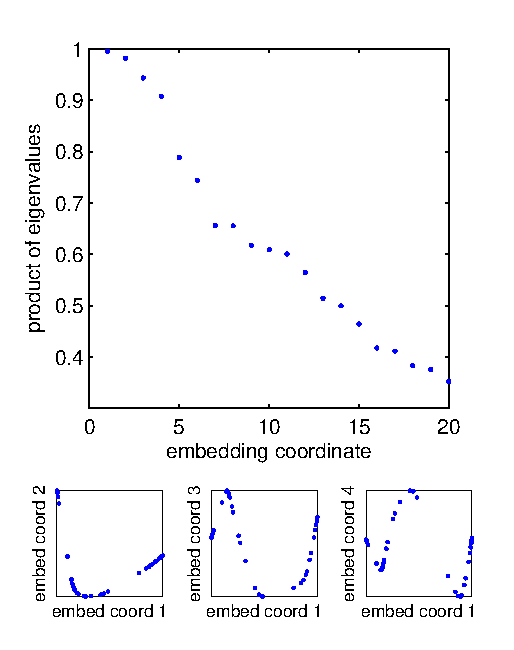
\includegraphics[width=\textwidth]{figS3}
\caption{}
\end{subfigure}
\begin{subfigure}{0.22\textwidth}
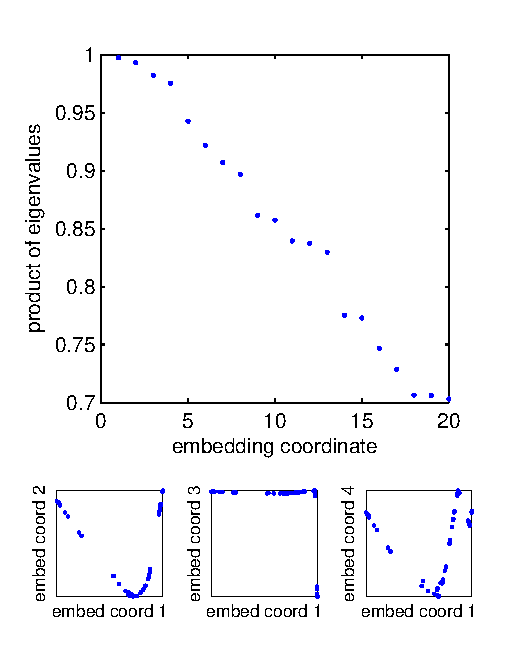
\includegraphics[width=\textwidth]{figS4}
\caption{}
\end{subfigure}
%
\begin{subfigure}{0.22\textwidth}
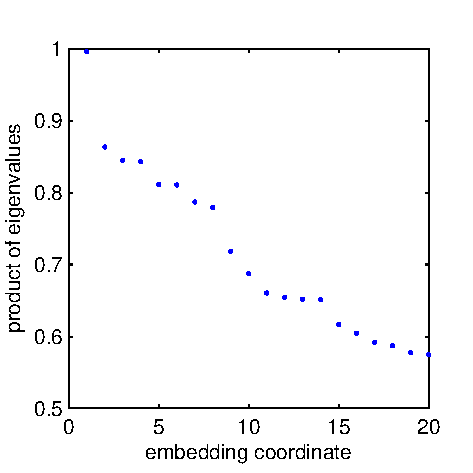
\includegraphics[width=\textwidth]{figS5}
\caption{}
\end{subfigure}
\begin{subfigure}{0.22\textwidth}
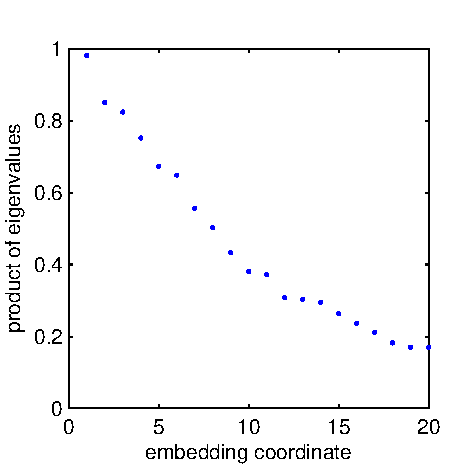
\includegraphics[width=\textwidth]{figS6}
\caption{}
\end{subfigure}
\caption[Eigenvalue spectra for imaging data sets]{Eigenvalue spectra for imaging data sets. (A) Eigenvalue spectrum for the {\em Drosophila} live imaging data set presented in \fig~3. Note that there is a gap after the fourth eigenvalue product. Below are the second, third, and fourth embedding coordinate plotted versus the first embedding coordinate. Note that coordinates 2--4 are higher harmonics (and thus simple functions) of coordinate 1, and are therefore not informative about structure in the data set.  We can conclude that the data set is effectively one-dimensional and can be parameterized/ordered by coordinate 1. (B) Eigenvalue spectrum for the zebrafish data set presented in \fig~4. Note that there is a gap after the fourth eigenvalue product. Below are the second, third, and fourth embedding coordinate plotted versus the first embedding coordinate. Note that coordinates 2--4 are higher harmonics (and thus simple functions) of coordinate 1, and are therefore not informative about structure in the data set.  It is not immediately obvious that coordinate 3 is a harmonic of coordinate 1; the distortion in the plot is due to density effects in the data (the developmental changes are slower towards the beginning of the trajectory, and so there is a higher density of images in this portion of the one-dimensional curve), We can conclude that the data set is effectively one-dimensional and can be parameterized/ordered by coordinate 1. (C) Eigenvalue spectrum for the fixed {\em Drosophila} images presented in \fig~5. Note that there is a gap after the first eigenvalue product. We can conclude that the data set is effectively one-dimensional and can be parameterized/ordered by coordinate 1. (D) Eigenvalue spectrum for the wing disc data set presented in \fig~6. Note that there is a gap after the first eigenvalue product. We can conclude that the data set is effectively one-dimensional and can be parameterized/ordered by coordinate 1. }
\label{fig:eigenvalues_images}
\end{figure}


\subsection{{\em Drosophila} embryo experiments}
%
Oregon-R was used as wild type {\em Drosophila} strains.
%
Embryos were collected and fixed at 22$^\circ$C.
%
Monoclonal rabbit anti-dpERK (1:100, Cell signaling) and rat anti-Twist (1:500, a gift from Eric Wieschaus) were used to stain proteins of interest.
%
DAPI (1:10,000, Vector Laboratories) was used to visualize nuclei, and Alexa Fluors (1:500, Invitrogen) were used as secondary antibodies.
%
Histone-RFP strain was used to obtain time-lapse movie of gastrulating embryos at 22$^\circ$C.
%
Live embryos were loaded to the microfluidic device with PBST to keep them oxidized, and fixed embryos were loaded with 90\% glycerol.

%\subsection{{\em Drosophila} embryo microscopy}
%
Nikon A1-RS scanning confocal microscope, and the Nikon 60x Plan-Apo oil objective was used to image {\em Drosophila} embryos.
%
Embryos were collected, stained, and imaged together under the same microscope setting.
%
End-on imaging was performed by using the microfluidics device described previously \citep{chung2010microfluidic}.
%
Images were collected at the focal plane $\sim$90~$\mathrm{\mu m}$ from the posterior pole of an embryo (see \fig~\ref{fig:DV_view}).

\begin{figure}
\centering
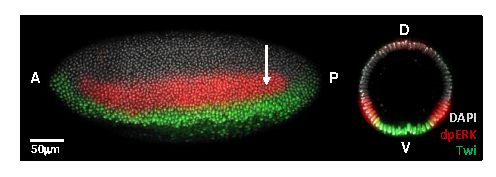
\includegraphics{figS1}
\caption[Lateral and cross-sectional views of {\em Drosophila} embryo]{(Left) A lateral view of a {\it Drosophila} embryo stained with DAPI (gray), dpERK (red), and Twi (green). The embryo is presented so that the anterior (A) side is to the left and the posterior (P) side is to the right. The arrow indicates the position where the cross-section of an embryo is imaged. (Right) A dorsoventral view of the cross-section of the {\it Drosophila} embryo. The dorsal (D) side is up and the ventral (V) side is down. Images were collected at the focal plane $\sim 18\%$ from the posterior pole of an embryo (arrow in the left image). }
\label{fig:DV_view}
\end{figure}





\section{Results}



\subsection{Method validation using live imaging}

\subsubsection{{\em Drosophila} gastrulation}

\begin{figure}[t]
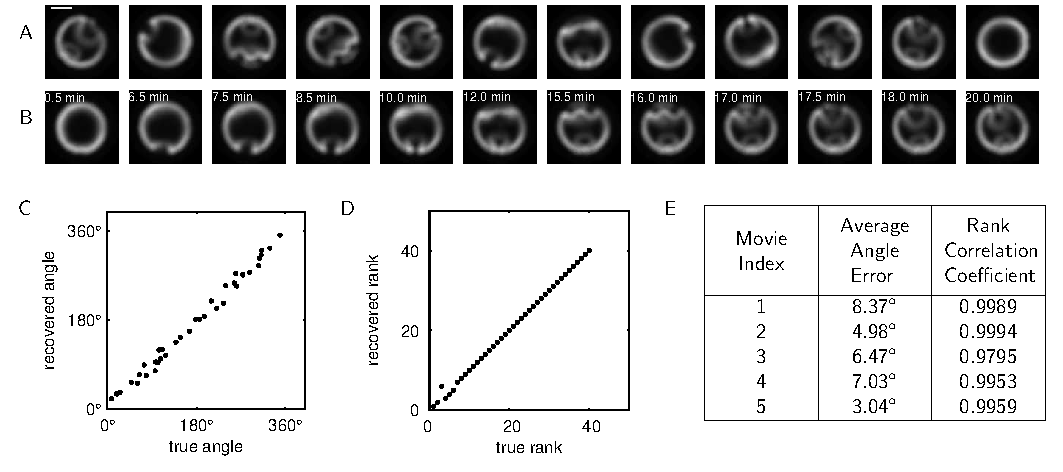
\includegraphics[width=\textwidth]{fig3}
\caption[Method validation using live imaging of \textit{Drosophila} embryos]{Method validation using live imaging of \textit{Drosophila} embryos. (A) Selected images from a live imaging study of a \textit{Drosophila} embryo during gastrulation. Scale bar indicates 50$\mu$m. Each frame is in an arbitrary rotational orientation, and the order of the frames has been shuffled. (B) Images from A registered and ordered by vector diffusion maps. The dorsal side of each embryo now appears at the top of each image, and the ventral side appears at the bottom. (C) The correlation between the recovered rotation angle (using vector diffusion maps) and the true rotation angle. The average absolute error in the recovered angles is $8.37 ^\circ$. (D) The correlation between the recovered rank (using vector diffusion maps) and the true rank. The rank correlation coefficient is $0.9989$. (E) The average error in the recovered angle and the rank correlation coefficient for $5$ independent live imaging studies. }
\label{fig:drosophila_live_imaging}
\end{figure}

To validate the proposed approach, we first applied our algorithm to a data set where the true temporal order and rotational orientation of the images were known {\em a priori}.
%
This data set was obtained through live imaging near the posterior pole of a vertically oriented {\it Drosophila} embryo during the twenty minutes spanning the late stages of cellularization through early gastrulation.
%
During this time window, the ventral furrow is formed, where the ventral side buckles towards the center of the embryo, internalizing the future muscle cells and forming a characteristic ``omega'' shape.
%
Germband extension then causes cells from the ventral side to move towards the posterior pole of the embryo, and then wrap around to the dorsal side \citep{leptin2005gastrulation}.
%
At the end of this process, cells which were originally on the ventral and posterior side of the embryo find themselves on the dorsal side, causing a similar ``omega'' to appear on the dorsal side.

\fig~\ref{fig:drosophila_live_imaging}A shows selected images from this live imaging data set, which contains $40$ consecutive frames taken at $30$~second time intervals at a fixed position within a single embryo.
%
Each image shows an optical cross-section near the posterior pole of a vertically oriented developing embryo, with the nuclei labeled by Histone-RFP.
%
Each frame was arbitrarily rotated, and the order of the frames was scrambled.
%
The original image resolution is $512 \times 512$.
%
All images were subsampled to $100 \times 100$ pixels for analysis, as this was found to be a sufficient resolution to retain all of the major developmental features within the data set. 
%
Images were normalized, and then blurred with a filter of radius 5\% of the total image (5 pixels). 
%
Images were not mean-centered or rescaled, as the entire live imaging data set was approximately centered already.
%
The task is now to register these images and order them in time to reconstruct the developmental trajectory.

We used vector diffusion maps to register and order the images.
%
\fig~\ref{fig:drosophila_live_imaging}B shows the images from \fig~\ref{fig:drosophila_live_imaging}A, now registered and ordered; the real time for each frame is also indicated.
%
With a small number of exceptions, the recovered ordering is consistent with the real time dynamics.
%
\fig~\ref{fig:drosophila_live_imaging}C and \fig~\ref{fig:drosophila_live_imaging}D  show the correlations between the recovered and true angles and rank orders, respectively, for the entire data set.
%
Both the angles and the ranks are recovered with a high degree of accuracy.
%
We note that determining which end of the trajectory corresponds to early in the developmental progression is a post-processing task that requires some {\em a priori} information. 

To assess the robustness of the proposed methodology, we repeated this procedure with four additional data sets extracted from independent live imaging studies spanning the same developmental time period.
%
The results are shown in \fig~\ref{fig:drosophila_live_imaging}E.
%
The errors in the recovered angles are all less than 10$^\circ$, and the rank correlation coefficients are consistently greater than 95\%, indicating that our methodology can reproducibly order data of this type.


\subsubsection{Zebrafish epiboly}

\begin{figure}[t]
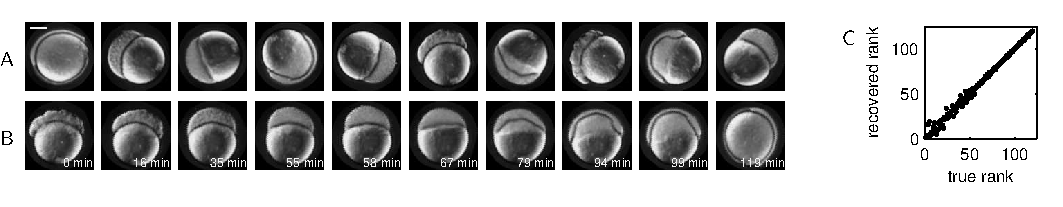
\includegraphics[width=\textwidth]{fig4}
\caption[Method validation using live imaging of a zebrafish embryo]{Method validation using live imaging of a zebrafish embryo. (A) Selected images from a movie of zebrafish epiboly. Scale bar indicates 200$\mu$m. Each frame is in an arbitrary rotational orientation, and the order of the frames has been shuffled. (B) Images from A after registration and ordering using vector diffusion maps. The real time of each frame is also indicated. (C) Correlation between the rank recovered using vector diffusion maps and the true rank.  The rank correlation coefficient is $0.9954$. The larger errors in the recovered ranks towards the beginning of the trajectory are due to the slow cell movement within that time window. }
\label{fig:zebrafish}
\end{figure}

As another validation for the proposed methodology, we applied our algorithm to a time-lapse movie  of zebrafish embryogenesis.
%
We used a publicly available live imaging data of zebrafish embryogenesis (\url{https://zfin.org/zf\_info/movies/Zebrafish.mov}) \cite{karlstrom1996flipbook}.
%
Taken with a differential interference contrast (DIC) microscope, the movie records the first $17$~hours of zebrafish development, from a single cell stage to a 16-somite stage.
%
We selected $120$ consecutive frames from this movie which capture 5.5~hours of epiboly (3.5--9~hours after fertilization).
%
The original image resolution was $320 \times 288$.
%
A $16$-pixel border was removed from the left and right sides to make the images square, and all images were then subsampled to $100 \times 100$ pixels for analysis, as this was found to be a sufficient resolution to retain all of the major developmental features within the data set. 
%
Images were not normalized or blurred.
%
Images were mean-centered so that the embryo in each frame was (approximately) centered. 
%
Images were not rescaled for size, as changes in overall size are important. 

In this experiment, embryos were immobilized for imaging so that the position and orientation remained fixed \citep{kane1996zebrafish}.
%
At the start of the time window, cells have divided 10--11 times and are accumulated in a cell mass above the yolk.
%
The cell mass is then compressed and the animal-vegetal axis of the embryo (vertical axis in \fig~\ref{fig:zebrafish}) shortens to form a spherical embryo shape by the end of the fourth hour of development.
%
Then, the yolk syncytial layer, which forms the boundary between the yolk and the cell mass, moves upward, forming a dome-shaped structure.
%
During this stage, the cells rearrange to form a uniform layer about four cells thick.
%
With time, this cell layer then spreads over across the yolk and expands toward the vegetal pole.
%
At the end of epiboly, the blastoderm completely engulfs the yolk.

As in the example of {\em Drosophila} embryo live imaging, the two-dimensional frames were randomly rotated and shuffled (\fig~\ref{fig:zebrafish}A).
%
We then used vector diffusion maps to register and order the frames.
%
The results are shown in \fig~\ref{fig:zebrafish}B.
%
The recovered rotations and order are consistent with the expected developmental dynamics, as shown in the correlations between the recovered and true ranks (\fig~\ref{fig:zebrafish}C).
%
Quantitatively, the rank correlation coefficient for this data set is 0.9954, and the average error in the recovered angle is $4.14^\circ$.
%
Some errors in ordering images of the early embryo result from slow cell movement during the early developmental stage where cells divide and accumulate above the yolk.
%
During epiboly, cell movement is more dynamic and the recovered ordering is more consistent with the real dynamics.

In summary, we have shown that our approach to temporal ordering performs very well on imaging data of two different developmental processes ({\em Drosophila} gastrulation and zebrafish epiboly), taken with two different imaging methods (fluorescent microscopy and DIC) where the true temporal order is known {\em a priori}.
%
Provided there exist significant dynamics within the data set and that the developmental trajectory is well-sampled, the developmental dynamics can be recovered.

\subsection{Data sets with intersample variability}

\subsubsection{Fixed images of {\em Drosophila} gastrulation}


We have analyzed how our algorithm performs on two model data sets where all images come from a single embryo.
%
In practice, we are interested in cases where each image comes from a different embryo, and the largest source of noise in the considered data set arises from embryo-to-embryo variability.
%
To demonstrate that our methods are robust to such variations,
we constructed a synthetic time course data set by selecting a random image from one of five {\em Drosophila} live imaging data sets (those data sets used in \fig~\ref{fig:drosophila_live_imaging}) at each time point.
%
The resulting data set is spatially unregistered, scrambled in time, and reflects embryo-to-embryo variability.
%
The median rank correlation coefficient when ordering such a synthetic time course using our methodology was 0.77, indicating that the algorithm can recover the temporal order even under noisy conditions.

We then applied our approach to a data set where the true rotational orientation and temporal order was not known {\it a priori}.
%
\fig~\ref{fig:drosophila_fixed_images}A shows selected images from a set of $120$ images of developing {\em Drosophila} embryos which cover a thirty minute time interval spanning late cellularization through gastrulation.
%
This data set is more complex than the live imaging data sets in that it contains significantly more images, each of which provides information about tissue morphology and the spatial distribution of two regulatory proteins.
%
Each image shows an optical cross-section of the posterior view of a {\em different} embryo at a different rotational orientation and fixed at a different (and unknown) developmental time.
%
The nuclei (gray) were labeled with DAPI, a DNA stain.
%
Embryos were stained with the antibody that recognizes Twist (Twi, shown in green), a transcription factor which specifies the cells of the future muscle tissue.
%
Another signal is provided by the phosphorylated form of the extracellular signal regulated kinase (dpERK, shown in red), an enzyme that, in this context, specifies a subset of neuronal cells \citep{Lim2013kinetics}.

The original image resolution was $1024 \times 1024$.
%
All images were subsampled to $100 \times 100$ pixels for analysis, as this was found to be a sufficient resolution to retain all of the major developmental features within the data set. 
%
The nuclei channel was normalized, and all channels were blurred with a filter of radius 5\% of the total image (5 pixels) to remove the effects of individual nuclei. 
%
The nuclei channel was scaled by half; because this signal occupies a larger fraction of the image relative to the other signals, its overall contribution is large, and so we downscaled it so that each signal would have more comparable weight in the algorithm. 
%
The images were mean-centered and scaled to have a constant size using the nuclei signal to detect the edges of the embryo within the frame.
%
\fig~\ref{fig:drosophila_fixed_images}B shows the selected images in \fig~\ref{fig:drosophila_fixed_images}A, now registered and ordered using vector diffusion maps.
%
Registered and ordered images of individual embryos can then be used to construct a representative average trajectory. 
%
Each snapshot in the average trajectory is the (weighted) average of a group of successive images from the registered and ordered data set (see \sec~\ref{sec:smooth_traj}).
%
Averaging successive images removes some of the interembryo variability, so that sequential snapshots of this averaged trajectory, shown in \fig~\ref{fig:drosophila_fixed_images}C, serve as a summary of the stereotypic developmental dynamics.

\begin{figure}[t]
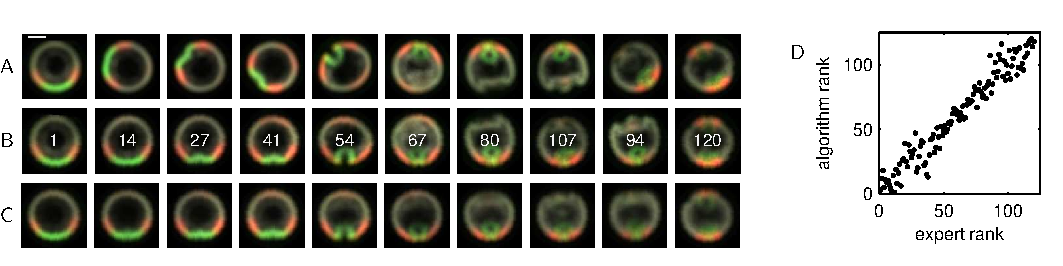
\includegraphics[width=\textwidth]{fig5}
\caption[Analysis of images of fixed \textit{Drosophila} embryos]{Analysis of images of fixed \textit{Drosophila} embryos. {(A)} Images of \textit{ Drosophila} embryos, stained for nuclei (gray), Twi (green), and dpERK (red). Scale bar indicates approximately 50$\mu$m (images have been rescaled to remove slight interembryo size variations).  Each image is of a different embryo arrested at a different developmental time and in a different rotational orientation. {(B)} Data from {\it A}, registered and ordered using vector diffusion maps. The expert rank for each image is indicated. {(C)} A representative ``developmental trajectory'' obtained from local averaging of the entire set of registered and ordered images (see \sec~\ref{sec:smooth_traj}). {(D)} Correlation between the image ranks calculated from the vector diffusion maps algorithm and the ranks obtained from ordering by an expert. The rank correlation coefficient is $0.9716$. }
\label{fig:drosophila_fixed_images}
\end{figure}


From this average trajectory, we can now easily see the developmental progression consistent with the known dynamics:
%
dpERK first appears as two lateral peaks at the ventrolateral side of the embryo, and a third dpERK peak then appears at the dorsal side of the embryo.
%
During mesoderm invagination, the two ventrolateral dpERK peaks merge together, eventually forming, together with Twi, the ``omega'' shape.
%
The dorsal dpERK peak then disappears during germband extension as cells from the ventral side wrap around to the dorsal side.
%
At the end of this process, similar ``omegas'' formed by Twi and dpERK appear on the dorsal side of the embryo; these patterns are most readily seen in the last image of \fig~\ref{fig:drosophila_fixed_images}C.
%
Thus, vector diffusion maps can accomplish the tasks presented in the caricature in \fig~\ref{fig:fish}, even in the absence of information about image landmarks and without {\it a priori} knowledge of developmental features.

To evaluate the quality of our registration and ordering, we can use prior knowledge about the developmental system.
%
The Twi signal is known to form a single peak at the ventralmost point of the embryo.
%
We found that the standard deviation in the location of this peak in the set of registered images was $\sim$8$^\circ$,
indicating that the algorithm successfully aligns the ventralmost points of the images.
%
Because the developmental time of each embryo cannot be easily estimated, we have few options for evaluating the quality of our temporal ordering.
%
We compared the ordering obtained from vector diffusion maps to the ordering provided by a trained embryologist who is knowledgeable about the developmental progression and the important image features.
%
The ranks from the ordering provided by the embryologist, which we will refer to as the ``expert rank'', are indicated for the images in \fig~\ref{fig:drosophila_fixed_images}B , and the rank correlation (see \fig~\ref{fig:drosophila_fixed_images}D) shows that our ordering is consistent with the expert ordering.


\subsubsection{Fixed z-stacks of {\em Drosophila} wing discs}

\begin{figure}[t]
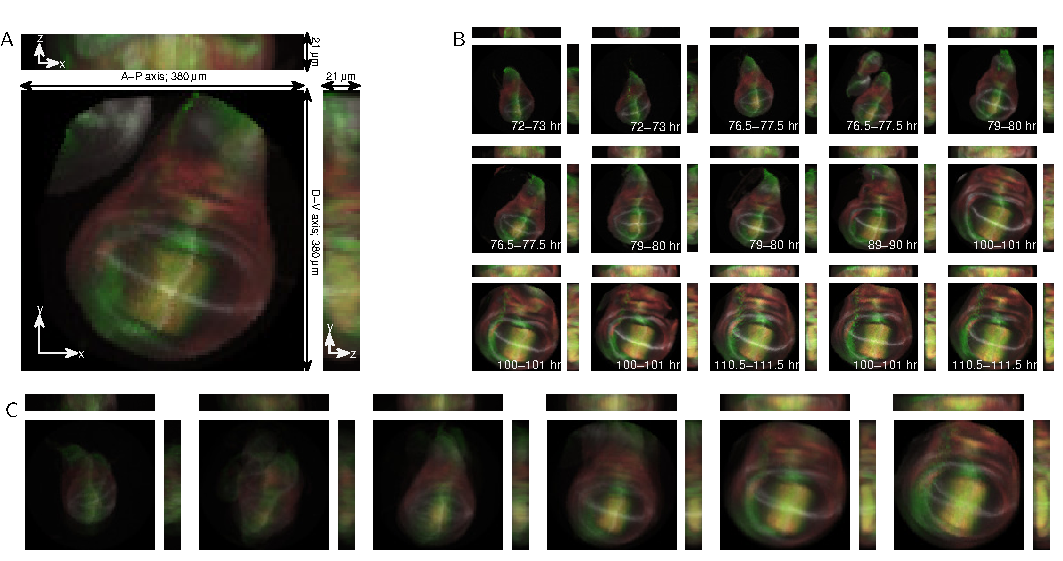
\includegraphics[width=\textwidth]{fig6}
\caption[Analysis of three-dimensional {\em Drosophila} wing disc z-stacks]{Analysis of three-dimensional {\em Drosophila} wing disc z-stacks. (A) Maximum projections of an example three-dimensional {\em Drosophila} wing disc z-stack. The anterior-posterior (A-P) and dorsal-ventral (D-V) axes are indicated. Discs express the Dad-GFP reporter construct (green), and are stained for Spalt (red), Wingless (gray), and Patched (gray). Projections along the $x$-, $y$-, and $z$-axes are shown. (B) Example three-dimensional images, ordered using diffusion maps. The time cohort, as assessed by an expert, is indicated for each image, and the rank correlation coefficient between the diffusion maps ordering and the expert timing is 0.9427. (C) The average developmental trajectory for the registered and ordered images. }
\label{fig:wing_disc}
\end{figure}

In this section we show that the approach can readily be applied to three-dimensional data. 
%
We restrict ourselves to the case where an obvious fixed axis exists, so that only rotations of the three-dimensional data around this axis need be taken into account.  
%
This does not constitute an inherent limitation for vector diffusion maps. 
%
While for simplicity here we will not discuss the general  case, incorporating general 3D symmetries is possible \citep{arie2012global, wang2013exact, cucuringu2012eigenvector}. 

To demonstrate this approach, we used an existing three-dimensional data set of fixed {\em Drosophila} wing imaginal discs \citep{hamaratoglu2011dpp}.
%
Imaginal discs are groups of progenitor cells in fly larva that will transform into specific organs during metamorphosis.
%
The wing disc is an imaginal disc that gives rise to the wing, thorax, and hinge.
%
The data set is composed of 46 fixed wing discs whose developmental times range from 72 to 112~hours after fertilization.
%
The original image resolution was $1024 \times 1024$.
%
Each of the original wing disc z-stacks contains 30--40 images taken at 1~$\mu$m intervals. 
%
All images were subsampled to $100 \times 100$ pixels for analysis, as this was found to be a sufficient resolution to retain all of the major developmental features within the data set. 
%
Each wing disc z-stack was reduced to a 21-image stack, consisting of the brightest image and the 10 images above and below.
%
No channels were normalized or blurred in the images, and the channel intensities were kept at their imaging values. 
%
Images were mean-centered using the Wingless/Patched signal to detect the edges of the sample. 
%
Images were not rescaled for size, as changes in overall size are important. 

The discs were dissected from larvae expressing the Dad-GFP reporter construct (green) and stained with antibodies that recognize Spalt (red), Wingless (gray), and Patched (gray), the factors that play important roles in disc patterning and growth (\fig~\ref{fig:wing_disc}A).

In the wing disc, the anterior-posterior and dorsal-ventral axes are significantly larger than the third principal axis (see \fig~\ref{fig:wing_disc}A). 
%
Therefore, we need not consider registration in all three dimensions, and can instead focus on registering the wing discs with respect to rotations only in the x-y plane.
%
To register the data, we first aligned the maximum intensity projections using angular synchronization.
%
We then used these rotations to register the full three-dimensional data in the x-y plane.
%
Because the maximum intensity projections are two-dimensional images, this step is no more computationally intensive than the previous examples.
%
Such an approach is possible when there are distinct major and minor axes within a three-dimensional sample, which reduces the rotational degrees of freedom.

We then used diffusion maps to order the registered three-dimensional data.
%
\fig~\ref{fig:wing_disc}B shows selected images from the data set ordered by diffusion maps.
%
In the original data set, each disc was assigned to one of six time classes (72--73~hr, 76.5--77.5~hr, 79--80~hr, 89--90~hr, 100--101~hr, and 110.5--111.5~hr after fertilization) by an expert; these times are indicated in \fig~\ref{fig:wing_disc}B.
%
In the ordered set, the size of wing disc grows, and the intensity of the Dad-GFP signal increases as a function of time.
%
The rank correlation coefficient based on the time class is 0.9436.
%
The registration errors are primarily due to some wing discs having extra tissue attached to them (such as the image in \fig~\ref{fig:wing_disc}A and the fourth image in \fig~\ref{fig:wing_disc}B).
%
Even with such obstructions, we can accurately order the images and extract a stereotypical developmental trajectory, shown in \fig~\ref{fig:wing_disc}C, by averaging (see \sec~\ref{sec:smooth_traj}).
%
We can now clearly see the growth of the wing disc, even though averaging somewhat blurs some finer scale structures.


\subsection{Computational requirements}

\begin{figure}[t]
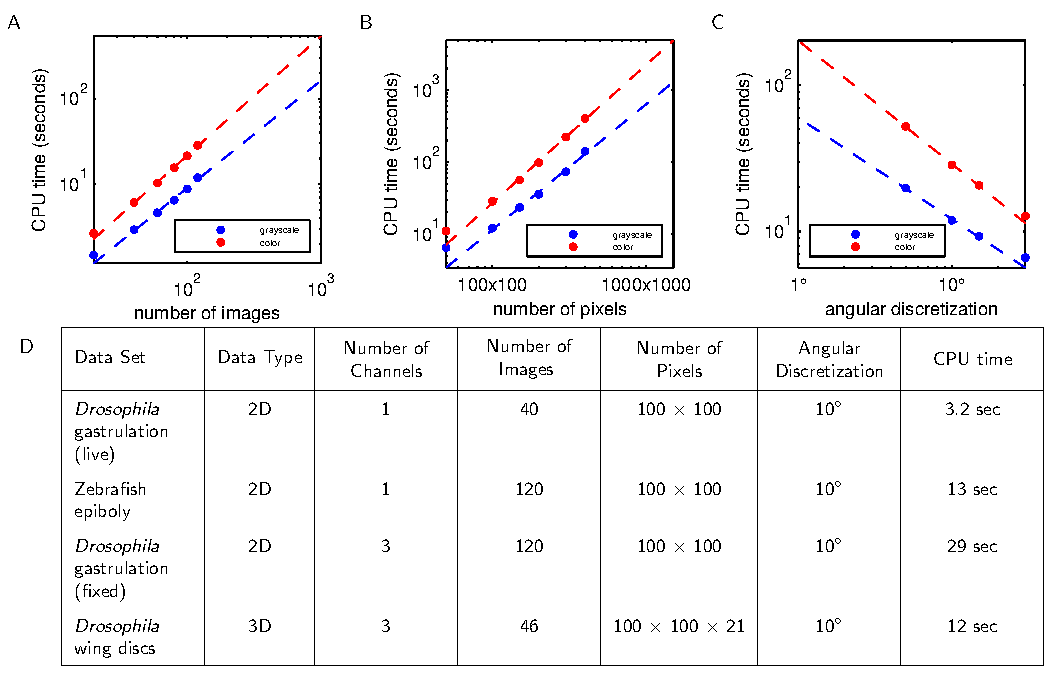
\includegraphics[width=\textwidth]{fig7}
\caption[Computational requirements for registration and ordering of biological images]{Computational requirements for the presented methodology. (A) CPU time as a function of the number of images in the data set (for $100 \times 100$ pixel images, and $10^\circ$ angular discretization). Empirically, the CPU time is $\sim \mathcal{O}(n^{1.33})$ in number of images. (B) CPU time as a function of the number of pixels in the images (for $120$ images, and $10^\circ$ angular discretization). Empirically, the CPU time is $\sim \mathcal{O}(n^{1.83})$ in the number of pixels. (C) CPU time as a function of the number of rotations (for $120$ images of $100 \times 100$ pixels). Empirically, the CPU time is $\sim \mathcal{O}(n^{-0.77})$ in the angular discretization. (D) The algorithm settings and computational requirements for the data sets analyzed. All times are reported for an Intel Core i7 2.93 GHz processor.}
\label{fig:cpu_time}
\end{figure}


The computational costs for our methodology are outlined in \fig~\ref{fig:cpu_time}.
%
The computational time is a function of the number of images in the data set, the number of pixels in each point, and the angular resolution to compute the pairwise rotations.
%
Furthermore, the computation of the pairwise rotational alignments, which accounts for the majority of the computational time, is trivially parallelizable, and only a subsample of the pairwise alignments need to be computed for larger data sets for accurate recovery of the underlying rotations \citep{singer2011angular}.
%
Because the computational cost increases with the image resolution, we chose to subsample all of our data sets to $100 \times 100$ pixels.
%
This resolution allowed us to rapidly analyze our data sets while still retaining all of the relevant developmental features.
%
However, as can be seen from the computational costs in \fig~\ref{fig:cpu_time}, it is feasible to use our algorithms to analyze higher-resolution images.

The requisite user intervention and parameter tuning required for our method is relatively minor.
%
As a first step, images must be preprocessed so that the Euclidean distance between the pixels is informative.
%
Our software provides several preprocessing options (such as blurring, rescaling, and mean-centering), as well as some guidance for what options to select depending on the system of interest.
%
Two algorithmic parameters, the angular discretization to compute the pairwise alignments and the diffusion maps kernel scale which determines which data points are ``close'' (see ~\fig~\ref{fig:schematics}), must also be defined.
%
We also provide some guidance on selecting these parameters, and found that the results are robust to both of these parameters.
%
Overall, the tasks of image preprocessing and parameter selection are relatively simple compared to manual registration and ordering of images, and so this methodology is promising for much larger imaging data sets which are impractical to evaluate manually.

\section{Discussion}

\begin{table}
\caption[PCA and vector diffusion maps comparison]{Comparison between rank correlation coefficients when ordering using the first vector diffusion maps (VDM) embedding coordinate, and rank correlation coefficients when ordering by the first principal component analysis (PCA) \citep{shlens2005tutorial} projection coefficient. For ordering using PCA, we computed the first principal component of the registered images, and then ordered the images by the projection coefficients onto this first mode. The PCA ordering is always less accurate than the vector diffusion maps ordering. In the zebrafish data set, the ordering is much less accurate using PCA, as the dynamics of the morphing and spreading of the cell mass are highly nonlinear. The PCA and VDM orderings are comparable for the wing disc data; this is to be expected, as the tissue simply grows in time.  }\textsf{
\begin{tabular}{| r | c | c |}
\hline
Data set & \parbox[c]{4cm}{ \centering VDM Rank Correlation} & \parbox[c]{4cm}{ \centering PCA Rank Correlation} \\
\hline
{\em Drosophila} gastrulation (live) & 0.9989 & 0.8137 \\
Zebrafish epiboly & 0.9955 & 0.6351 \\
{\em Drosophila} gastrulation (fixed) & 0.9716 & 0.8658 \\
{\em Drosophila} wing discs & 0.9436 & 0.9381 \\
\hline
\end{tabular}
}

\label{tab:PCA_compare}
\end{table}

Temporal ordering of large-scale data was done in the context of molecular profiling studies, in which data points are vectors describing the expression levels of different mRNA \citep{anavy2014blind, trapnell2014dynamics, gupta2008extracting}.
%
At the same time, temporal ordering of imaging data sets was done with a significant amount of human supervision and using registered images as a starting point \citep{yuan2014automated, surkova2008characterization, fowlkes2008quantitative}, or using some {\em a priori} knowledge of the relevant developmental processes \citep{dubuis2013accurate}.
%
In contrast to most of the existing registration approaches which rely on the knowledge of appropriate landmarks in the images \citep{ian1998statistical} (such as the eyes in face recognition applications \citep{zhao2003face}), algorithms based on angular synchronization can register images even in the absence of such information, making them relevant for a wide variety of applications.

Angular synchronization and vector diffusion maps have been used to reconstruct molecular shapes from cryo-electron microscopy images \citep{singer2012vector, zhao2014rotationally, singer2011viewing}.
%
Because of high levels of instrument noise in these data, thousands of images were needed for successful shape reconstruction.
%
Based on the presented results, we expect that much smaller data sets may be sufficient for successful reconstruction of developmental trajectories from snapshots of fixed tissues.
%
In general, the size of the data set required for accurate registration and ordering is a function of the instrument noise, interembryo variability, and the complexity of the developmental dynamics.

The benefits of our approach to image data mining are twofold.
%
First, the algorithm can accomplish the tasks of registration and ordering in a single step.
%
Furthermore, because our methodology is nonlinear, it can successfully order data sets which contain complex dynamics (see \tab~\ref{tab:PCA_compare} for a comparison of ordering using linear principal component analysis versus vector diffusion maps for the data sets presented in this paper).
%
We expect nonlinear techniques to be necessary for larger data sets which span a wider dynamic range.
%
The main utility of our proposed methodology lies in the analysis of data sets containing hundreds of images from systems which have not been well-studied.
%
For such data sets, manual ordering of the images can be nontrivial, and our algorithms can clearly accelerate uncovering the underlying developmental dynamics.

We acknowledge that our methods, though general, do have limitations.
%
The first is that we require enough data to sufficiently sample the developmental trajectory.
%
Therefore, for very small and/or very noisy data sets, our algorithms may fail.
%
Second, the pertinent image features need to be large compared to the noise and the image resolution.
%
In all of our examples, the relevant expression patterns and morphological structures span several pixels and are large compared to both the instrument noise and embryo-to-embryo variability, making the Euclidean distance between pixels a good measure of images similarity.

Vector diffusion maps allow us to automatically register images, an essential task for many applications.
%
Simultaneously, the algorithm provides us with parameters to describe each image.
%
In the examples presented here, we have focused on ordering the images in time using the first vector diffusion maps coordinate.
%
In general, we can recover several coordinates which concisely and comprehensively describe the data set.
%
This parametrization can then be used for typical data analysis tasks, such as outlier detection and model fitting.
%
Furthermore, images taken from different viewing directions can be analyzed, as the vector diffusion maps parametrization will organize the images according to the viewing angle \citep{singer2011viewing}.
%
Another direction for future work is related to the joint analysis of data sets provided by different imaging approaches, such as merging live imaging data of tissue morphogenesis with snapshots of cell signaling and gene expression from fixed embryos \citep{krzic2012multiview, ichikawa2014live, rubel2010coupling, dsilva2013nonlinear}.
%
It would also be interesting to explore the connections between our proposed approach and recently developed methods for ordering and classification of face images \citep{kemelmacher2011exploring, kemelmacher2014illumination}
%
Given the rapidly increasing volumes of imaging data from studies of multiple developmental systems, we expect that dimensionality reduction approaches discussed in this work will be increasingly useful for biologists and motivate future applications and algorithmic advances.

In the previous chapters, we have discussed using diffusion maps to analyze different types of data from dynamical systems (multiscale time series data, data collected via different measurements of the same systems, and imaging data collected in different orientation).
%
However, we have mostly ignored the issue of detecting the dimensionality of the underlying manifold.
%
Because of the issue of ``repeated eigendirections,'' where some diffusion maps coordinates are higher harmonics of previous coordinates and do not describe any new directions in the data, detecting how many and which coordinates one must retain is a difficult issue. 
%
In the next chapter, we will present a methodology to address this problem, which must be addressed for diffusion maps to be broadly applicable to the analysis of dynamical systems data. 
